% !TEX TS-program = xelatex
% !TEX encoding = UTF-8
\documentclass[11pt]{ctexart} 

\usepackage{geometry} % See geometry.pdf to learn the layout options. There are lots.
\geometry{a4paper} % or letterpaper (US) or a5paper or....

\usepackage{graphicx} % support the \includegraphics command and options
\usepackage{float}
\usepackage[bookmarks=true]{hyperref} %支持生成书签

\title{Computational Physics HomeWork 2}
\author{林祥}
%\date{} % Activate to display a given date or no date (if empty),
         % otherwise the current date is printed 

\begin{document}
\maketitle

\section{一维扩散问题}

\subsection{问题描述}

\begin{equation}
\left\lbrace 
\begin{array}{l}
\frac{\partial u}{\partial t}=\frac{\partial^{2}u}{\partial x^{2}} \indent (0\leq x\leq 1, 0<t)\\
u(0,t)=\sin (t),u(1,t)=0 \indent (0<t)\\
u(x,0)=0, \indent (0\leq x\leq 1) 
\end{array}
\right. 
\end{equation}
给出计算所用的离散化公式,计算流程,并绘制0<t<1时间范围内u(x,t)数据图

\subsection{基本方案}

分别对方程两边进行差分,得到显式FTCS公式如下

\begin{equation}
u(i,l+1)=u(i,l)+\lambda(u(i+1,l)-2u(i,l)+u(i-1,l))
\end{equation}

\indent 隐式FTCS公式如下

\begin{equation}
-\lambda u(i-1,l+1)+(1+2\lambda)u(i,l+1)-\lambda u(i+1,l+1)=u(i,l)
\end{equation}

\indent 其中下标i,l分别对应x,t, 取时间差分元 $ tau=0.0001 $ ,x差分元$ h=0.02 ,\lambda=\frac{tau}{h^2}=\frac{1}{4}<\frac{1}{2}$,
由于tau太小,实际画图时,每100个时间的数据取1组用来画图即可\\
\indent 对于显式公式,已知初始条件,可以直接由前一时刻求得下一时刻,另外考虑边界条件即可。\\
\indent 对于隐式公式,无法直接由上一时刻求得下一时刻,观察隐式公式发现,可以使用三对角矩阵追赶法来求解下一时刻的数据。
其中$a=-\lambda,b=1+2\lambda,c=-\lambda$,
特别地,考虑x=1处的边界条件,a[-1]=0(基于python,a数组最后一位为0),b[-1]=1,
考虑x=0处的边界条件,由于t相差0.0001,$\sin(t)$相差几乎为0,可令b[0]=1,c[0]=0,
求解完后需要对x=0处的u修正到准确值,防止误差放大。

\subsection{显式FTCS方法}

\begin{figure}[ht] %不加[h]将会导致插入图片位置出错
\centering
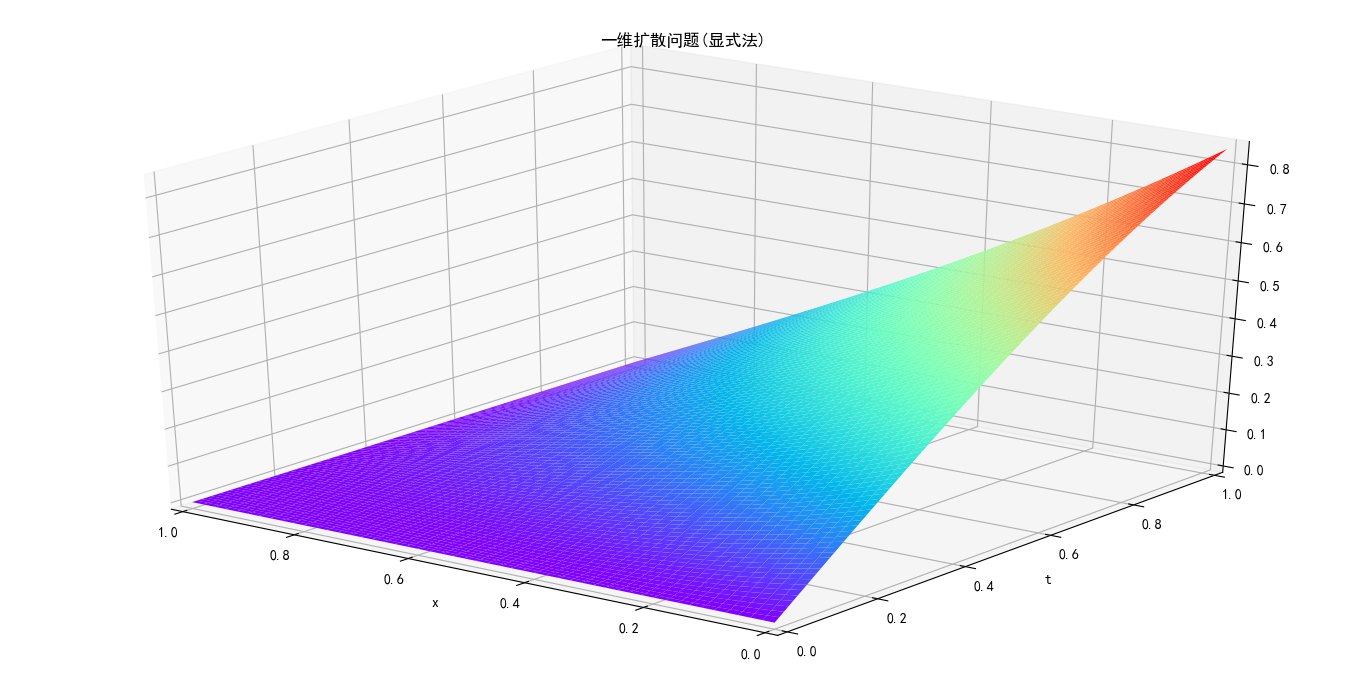
\includegraphics[width=0.8\linewidth]{Pyfingure/Figure_1_1.png} 
\caption{显式FTCS方法求解一维扩散问题}
\end{figure}

\subsection{隐式FTCS方法}

\begin{figure}[ht]
\centering
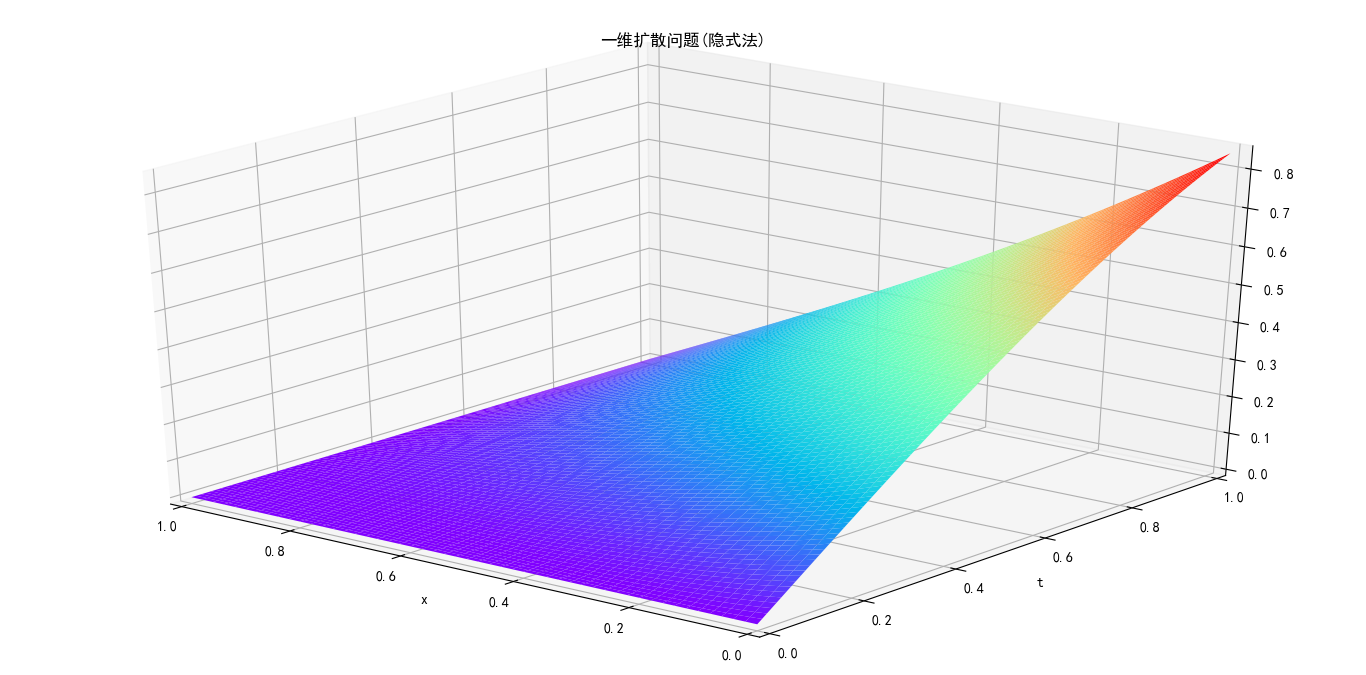
\includegraphics[width=0.8\linewidth]{Pyfingure/Figure_1_2.png} 
\caption{隐式FTCS方法求解一维扩散问题}
\end{figure}

\section{二维Laplace问题}

\subsection{问题描述}

\begin{equation}
\left\lbrace 
\begin{array}{l}
\frac{\partial^{2}u}{\partial x^{2}}+\frac{\partial^{2}u}{\partial y^{2}}=0 \indent (0<x<1, 0<y<1)\\
\mbox{边界条件}1\\
u(0,y)=0,u(1,y)=0 \indent (0\leq y\leq 1)\\
u(x,0)=0, u(x,1)=100 \indent (0\leq x\leq 1) \\
\mbox{边界条件}2\\
u(0,y)=0,u(1,y)=0 \indent (0\leq y\leq 1)\\
u(x,0)=0, u(x,1)=0 \indent (0\leq x\leq 1) \\
u(x,0.4)=-100,u(x,0.6)=100 \indent (0.3\leq x \leq 0.7)
\end{array}
\right. 
\end{equation}

给出计算所用的离散化公式,计算流程,给出计算结果的数据图。

\subsection{基本方案}

分别对方程两边进行差分,得到迭代公式如下
\begin{equation}
u(i,j)=(u(i+1,j)+u(i-1,j)+u(i,j+1)+u(i,j-1))/4
\end{equation}

\indent 为了提高迭代效率,减小迭代次数,实际程序采用超松弛迭代,公式如下
\begin{equation}
u(i,j)=\lambda(u(i+1,j)+u(i-1,j)+u(i,j+1)+u(i,j-1))/4+(1-\lambda)u(i,j)
\end{equation}
\indent 其中$\lambda $为超松弛因子,取为1.5\\
\indent 将xy平面网格化,每个网格点对应一个u值,x,y的差分元均为$h=0.01$,
在边界条件1下,$101\times 101$的数组u取边界条件的平均值作为迭代初值;边界条件2下,数组u取0作为迭代初值。取最大迭代次数为10000,容忍误差为1E-5.\\
\indent 按照公式(6)进行循环迭代,直到达到最大迭代次数,或满足容忍误差(前后两次计算的u数组的最大差值小于容忍误差),迭代结束。\\
\indent 特别地,对于边界条件2,除了考虑外围边界条件不变,还需保证y=0.4,和y=0.6处的u值不能修改(加入判断语句)。

\subsection{边界条件1下的电势分布}

经过2286次迭代后,达到容忍误差
\begin{figure}[ht]
\centering
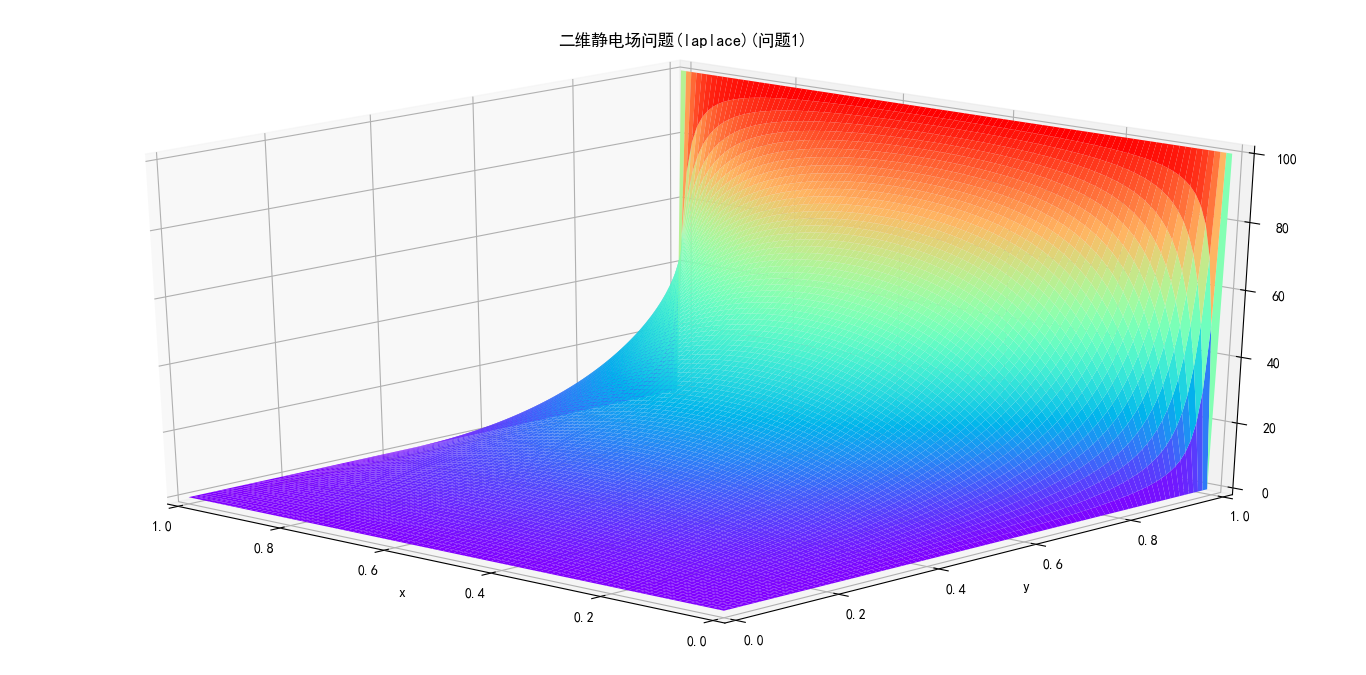
\includegraphics[width=0.8\linewidth]{Pyfingure/Figure_2_1.png} 
\caption{边界条件1下的电势分布}
\end{figure}

\subsection{边界条件2下的电势分布}

经过1070次迭代后,达到容忍误差
\begin{figure}[ht]
\centering
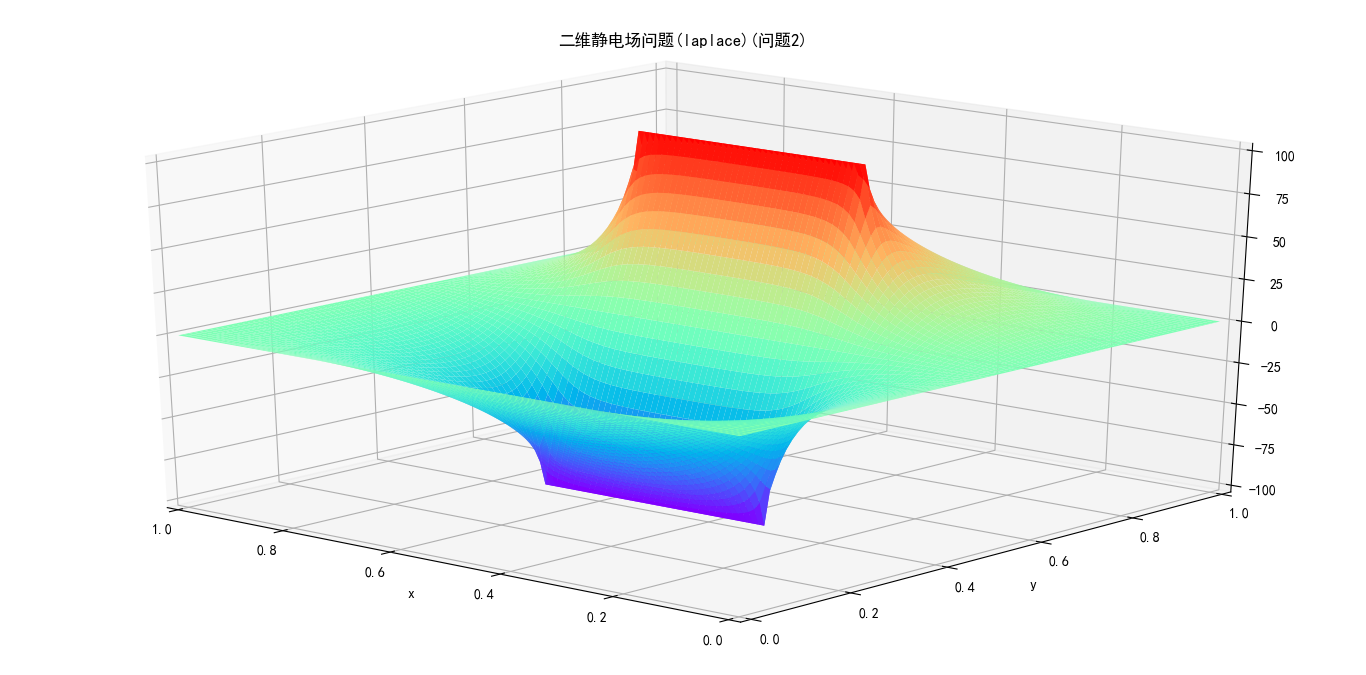
\includegraphics[width=0.8\linewidth]{Pyfingure/Figure_2_2.png} 
\caption{边界条件2下的电势分布}
\end{figure}

\section{一维波动方程问题}

\subsection{问题描述}

\begin{equation}
\left\lbrace 
\begin{array}{l}
\frac{\partial^{2}y}{\partial t^{2}}=v^{2}\frac{\partial^{2}y}{\partial x^{2}} \indent (0<x<1, 0<t)\\
y(0,t)=0,\frac{\partial y(1,t)}{\partial x}=0 \indent (0<t)\\
y(x,0)=\exp[-1000(x-0.3)^{2}], \indent (0\leq x\leq 1) \\
v=300,(0<x<0.5),\indent v=150,(0.5<x<1)
\end{array}
\right. 
\end{equation}

给出计算所用的离散化公式,计算流程,并绘制t=0, t=1E-3, t=1E-2时刻的波形图。

\subsection{基本方案}

分别对方程两边进行差分,得到递推公式如下
\begin{equation}
y(i,l+1)=-y(i,l-1)+(2-2\lambda^{2})y(i,l)+\lambda^{2}(y(i+1,l)+y(i-1,l))
\end{equation}
\indent 其中i,l分别对应x,t.取时间差分元$tau=1.25E-5$,x差分元$h1=0.005,h2=0.0025,\lambda_{1}=v_{1}*tau/h1=0.75,\lambda_{2}=v_{2}*tau/h2=0.75\in(\frac{\sqrt{2}}{2},1),\lambda$取值满足稳定性要求,但是相应的x在(0,0.5)和(0.5,1)步长是不一样的,需要特别注意。\\
\indent 定义一个三行的数组y,每行数据代表不同时刻y在x处的值,考虑到递推公式(8)中,要求下一时刻y值,需要知道前2个时刻的y值,我们假设存在时刻$t=-tau$,其对应的y值与$t=0$时刻y值相等,基于此按照时间递推即可求得下一时刻的y值,每次求完值之后,更新y数组,以便于求解下一时刻。\\
\indent 当然,递推过程中也需要保证边界条件; x=0处y值始终为0,x=1处y对x斜率为0,利用一阶近似,保证x=1处y值始终等于x=1-h处即可。

\subsection{不同时刻的波形图}

\begin{figure}[ht]
\centering
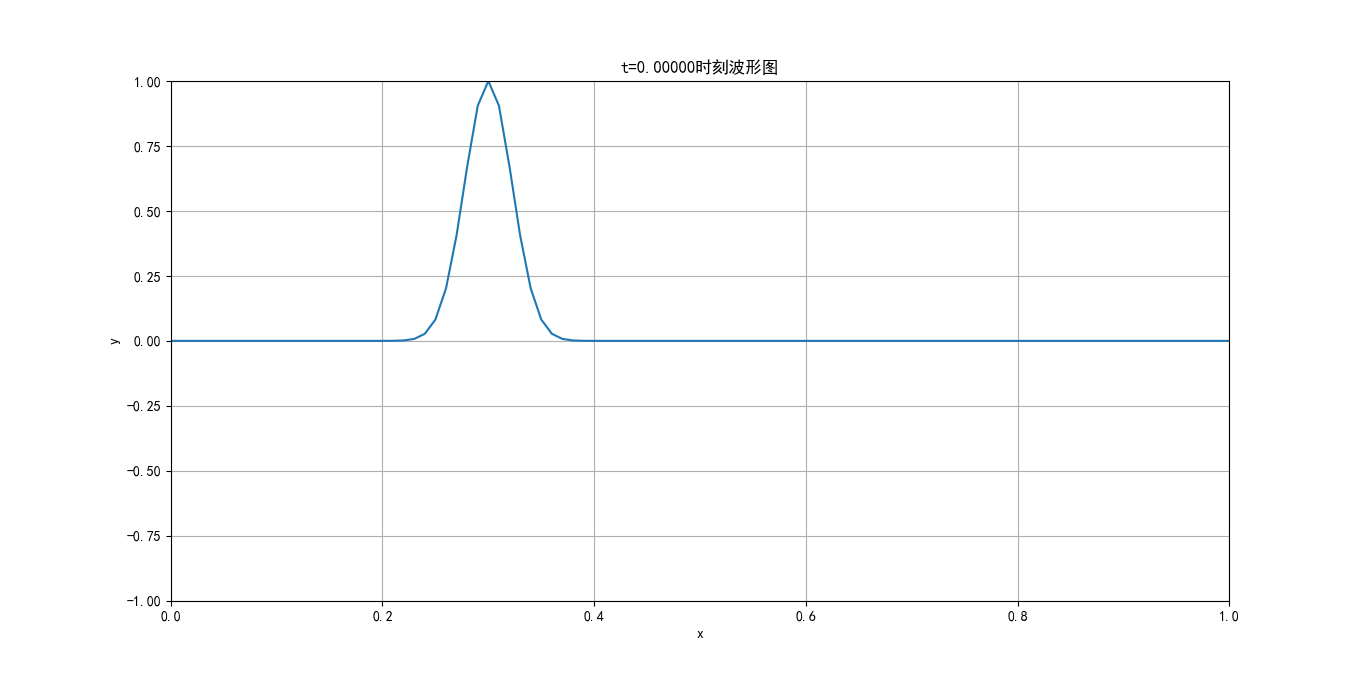
\includegraphics[width=0.8\linewidth]{Pyfingure/Figure_3_3.png} 
\caption{t=0时刻波形图}
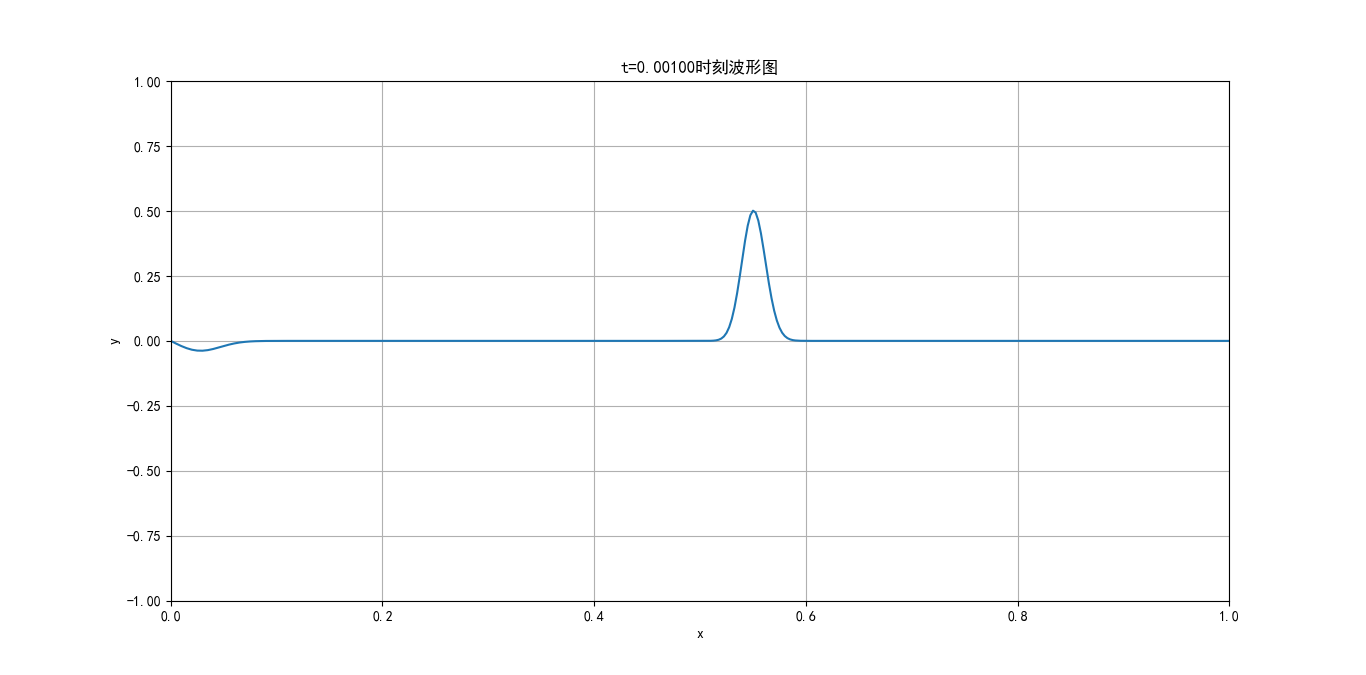
\includegraphics[width=0.8\linewidth]{Pyfingure/Figure_3_1.png} 
\caption{t=1E-3时刻波形图}
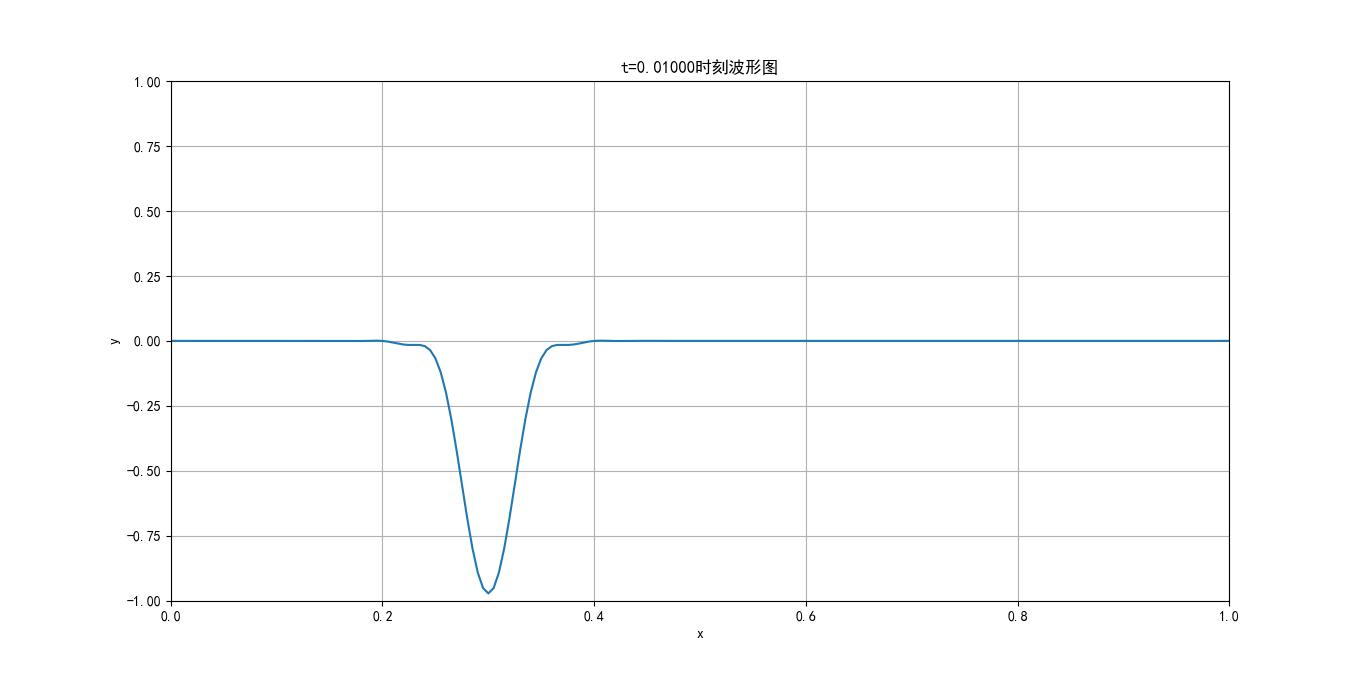
\includegraphics[width=0.8\linewidth]{Pyfingure/Figure_3_2.png} 
\caption{t=1E-2时刻波形图}
\end{figure}

\end{document}
